\documentclass[unknownkeysallowed]{beamer}

\mode<presentation> {
\usetheme{Madrid}
}

\usepackage{graphicx} % Allows including images
\usepackage{booktabs} % Allows the use of \toprule, \midrule and \bottomrule in tables

\usepackage[utf8]{inputenc}
\usepackage[slovene]{babel}
\usepackage{algorithmicx, algpseudocode}

\usepackage{varwidth}

\usepackage[labelformat=empty]{caption}
\addto\captionsslovene{\renewcommand{\figurename}{Figure}}

\def\R{\mathbb R}

%----------------------------------------------------------------------------------------
%	TITLE PAGE
%----------------------------------------------------------------------------------------

\title[Text Analysis]{Text classification using persistent homology} % The short title appears at the bottom of every slide, the full title is only on the title page

\author{Matija Čufar, Domen Keglevič} % Your name
\institute[] % Your institution as it will appear on the bottom of every slide, may be shorthand to save space
{
Faculty of Computer and Information Science \\ % Your institution for the title page
\medskip
}
\date{\today} % Date, can be changed to a custom date

%----------------------------------------------------------------------------------------
%	PRESENTATION
%----------------------------------------------------------------------------------------

\begin{document}

\begin{frame}
\titlepage % Print the title page as the first slide
\end{frame}

\begin{frame}
\frametitle{Problem description} 
\begin{block}{Problem}
\begin{columns}[c]
\column{.6\textwidth}
	Given sets of texts from different domains, build a classifier which can distinguish between the domains.
\column{.35\textwidth}
	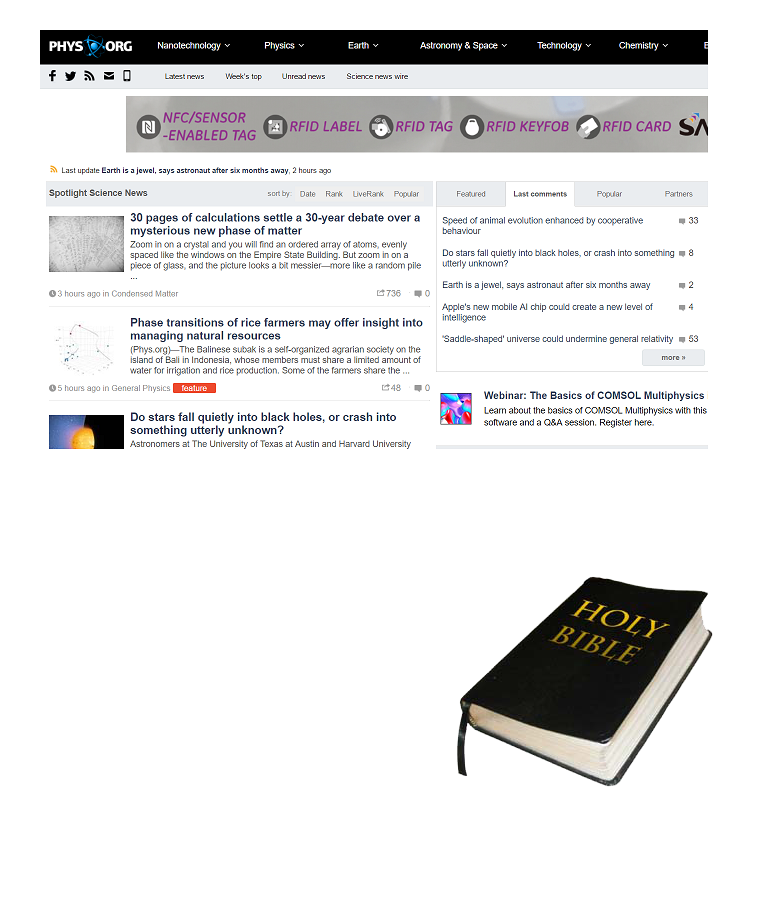
\includegraphics[width=0.9\linewidth]{different_domains}
\end{columns}
\end{block}
\end{frame}

\begin{frame}
\frametitle{Solution idea}
\begin{itemize}
\item Use persistent homology.
\bigskip
\item For each text calculate several features (get a vector in $\R ^d$).
\bigskip
\item Make a simplicial complex using distances between vectors of features.
\bigskip
\item Calculate bottleneck distance between persistence diagrams.
\end{itemize}
\end{frame}


\begin{frame}
\frametitle{Which features?}
We calculated several features:
\medskip
\begin{itemize}
\smallskip
\item Average word length / longest word length,
\bigskip
\item num of different words / num of all words,
\bigskip
\item three words with top tf-idf / num of all words,
\bigskip
\item etc.
\bigskip
\item Separately: distribution of word and sentence length.
%\bigskip
%\item num of words with at most eight chars / num of all words
%\bigskip
%\item num of words with at least nine chars / num of all words
%\bigskip
%\item average sentence length / longest sentence length
\end{itemize}

\end{frame}

\begin{frame}
\frametitle{Results}
Some barcodes:
\begin{columns}[c]
\column{.5\textwidth}
\begin{figure}
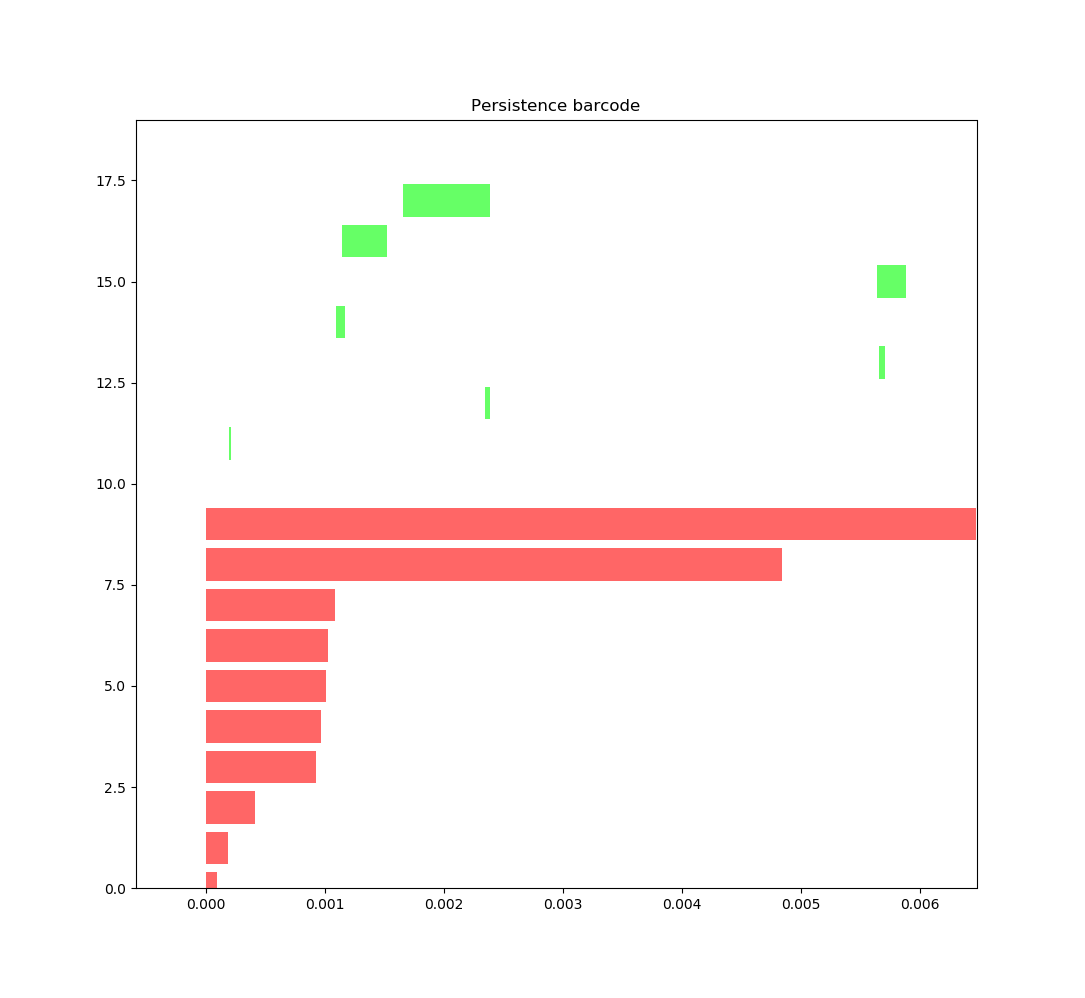
\includegraphics[width=0.9\linewidth]{../plots/barcodes/phys-b-all}
\caption{Physics news}
\end{figure}

\column{.5\textwidth}
\begin{figure}
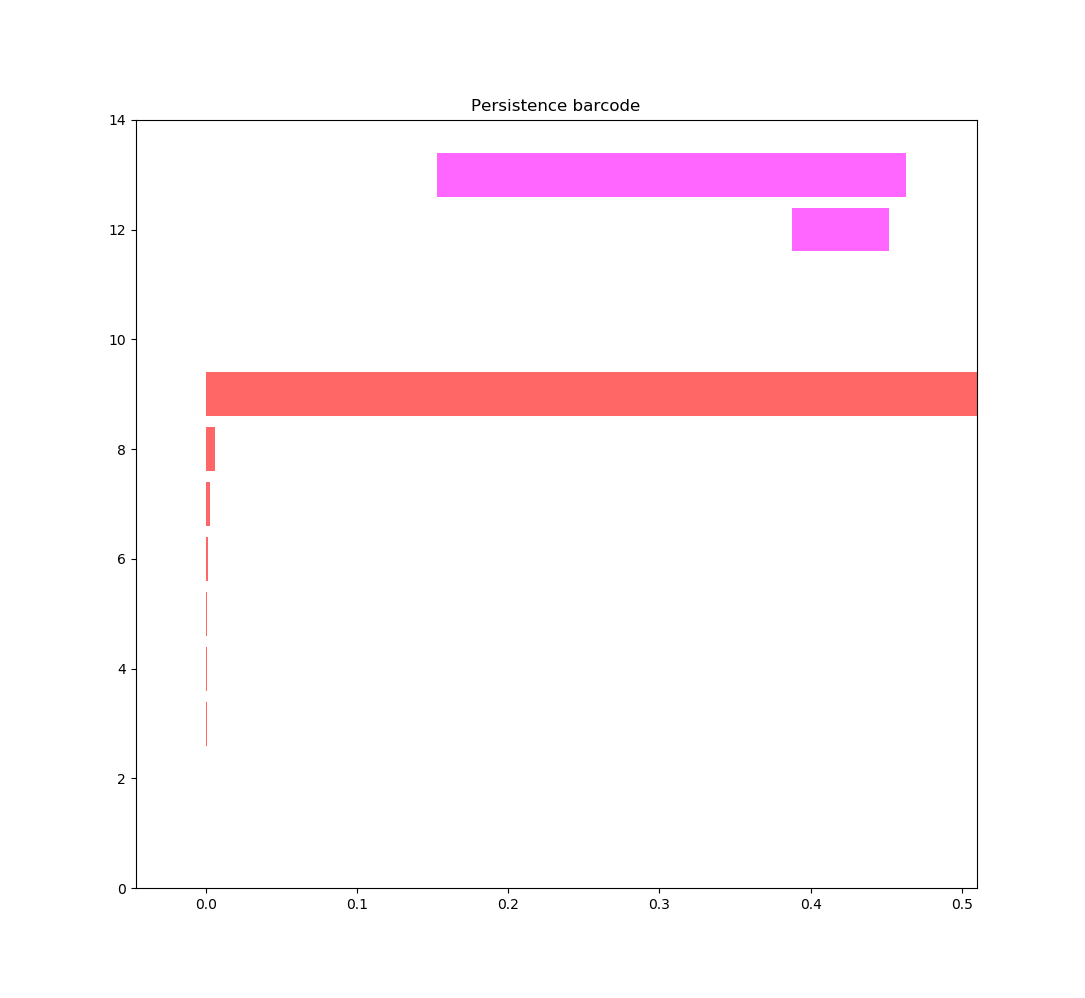
\includegraphics[width=0.9\linewidth]{../plots/barcodes/recipes-b-all}
\caption{Recipes}
\end{figure}

\end{columns}
\end{frame}


\begin{frame}
\frametitle{Results}
Some persistence diagrams:
\begin{columns}[c]
\column{.5\textwidth}
\begin{figure}
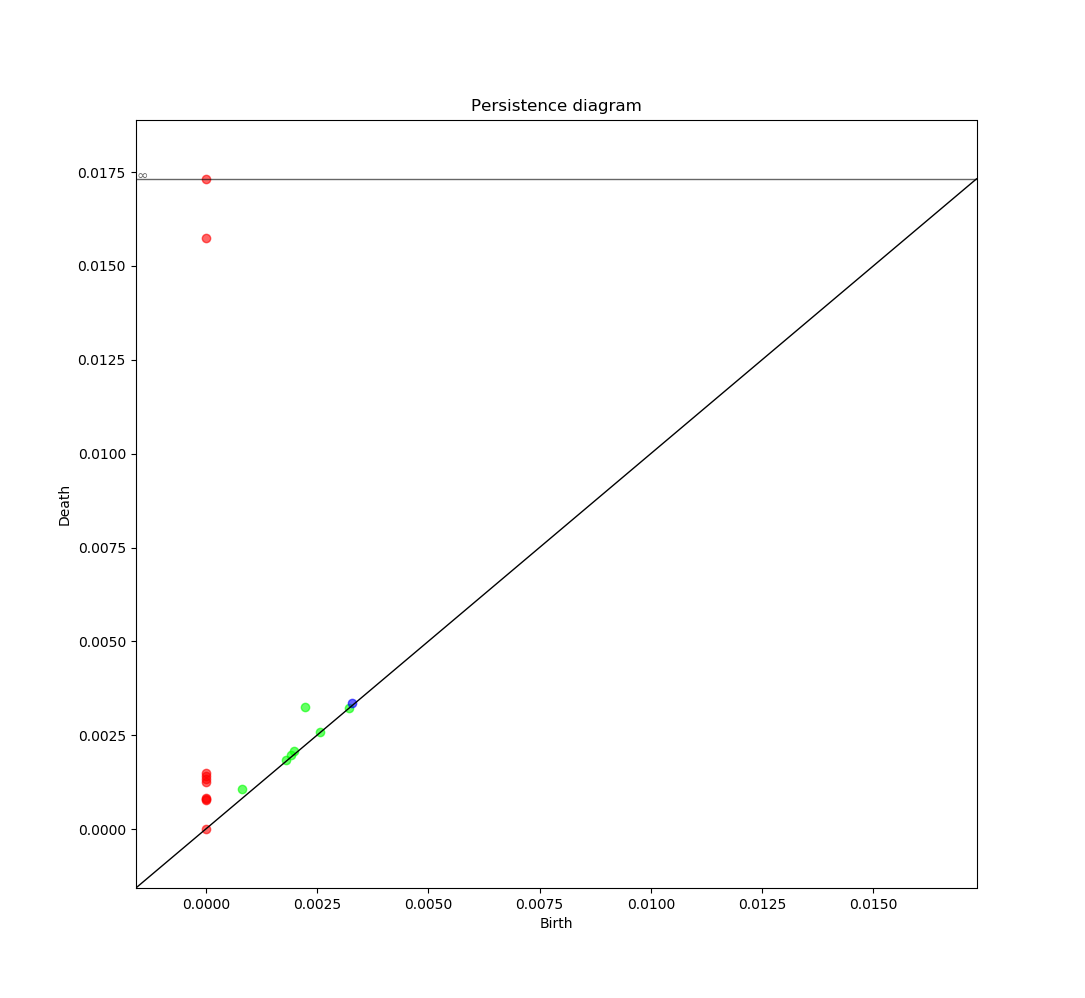
\includegraphics[width=0.9\linewidth]{../plots/diagrams/bible-new-d-all}
\caption{Bible, New Testament}
\end{figure}

\column{.5\textwidth}
\begin{figure}
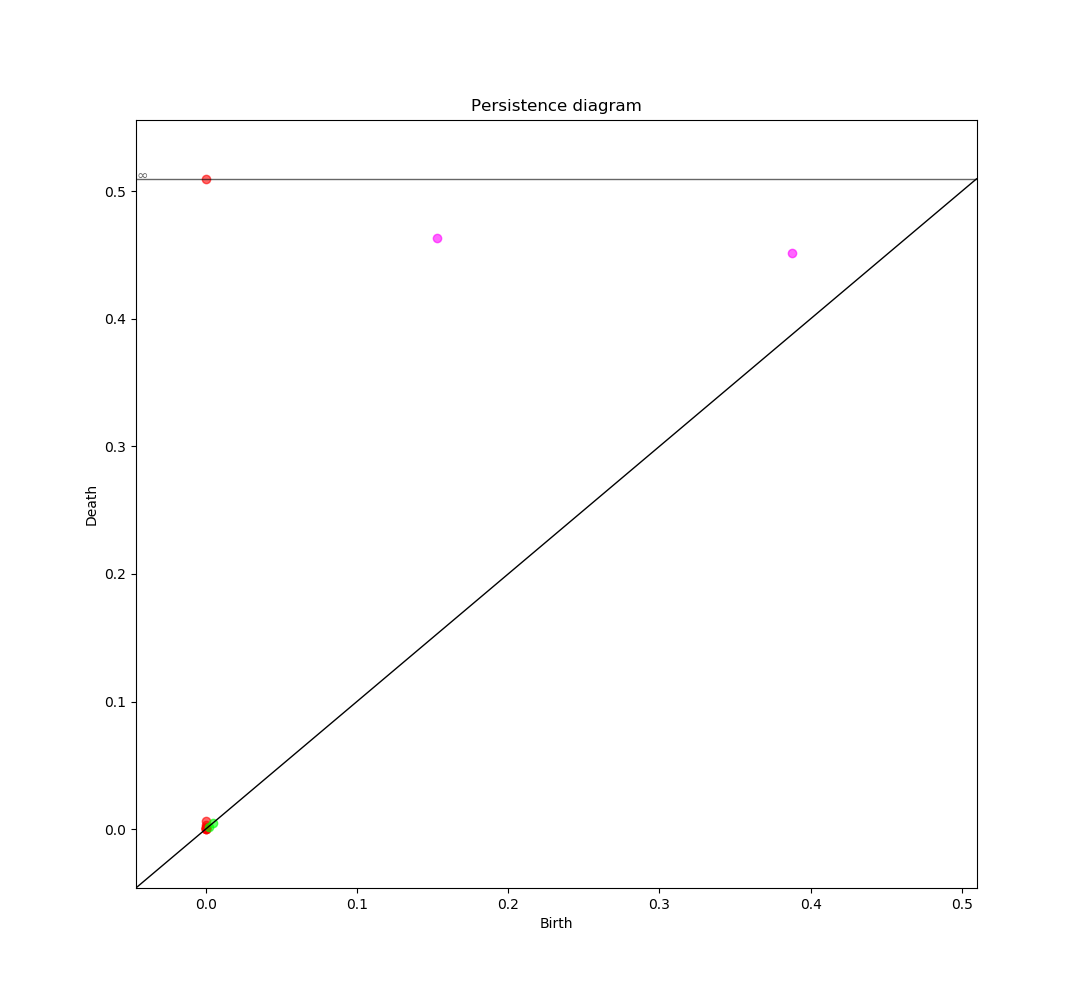
\includegraphics[width=0.9\linewidth]{../plots/diagrams/recipes-d-all}
\caption{Recipes}
\end{figure}

\end{columns}
\end{frame}


\begin{frame}
\frametitle{Results (vector of features)}
\bigskip
\begin{figure}
\begin{tabular}{ c c c c c c }
	& bible-new & recipes & phys.org & bible-old \\
  	\hline			
   bible-new & 0.000 & 0.008 & 0.008 & 0.008 \\
   recipes   & 0.008 & 0.000 & 0.002 & 0.003 \\
   phys.org  & 0.008 & 0.002 & 0.000 & 0.003 \\
   bible-old & 0.008 & 0.003 & 0.003 & 0.000 
\end{tabular}
\caption{Bottleneck distance (alpha complex, points in $\R ^d$)}
\end{figure}

\begin{figure}
\begin{tabular}{ c c c c c c }
	& bible-new & recipes & phys.org & bible-old \\
  	\hline			
  bible-new & 0.000 & 0.094 & 0.112  &  0.082 \\
  recipes   & 0.094 & 0.000 & 0.045  &  0.054 \\
  phys.org  & 0.112 & 0.045 & 0.000  &  0.082 \\
  bible-old & 0.082 & 0.054 & 0.082  &  0.000 
\end{tabular}
\caption{Bottleneck distance (Rips complex, points in $\R ^d$)}
\end{figure}
\medskip
\end{frame}

\begin{frame}
\frametitle{Results (histograms)}

\begin{figure}
\begin{tabular}{ c c c c c c }
	& bible-new & recipes & phys.org & bible-old \\
  	\hline 
  bible-new   & 0.000 & 0.109 & 0.250 & 0.185\\
  recipes     & 0.109 & 0.000 & 0.165 & 0.132\\
  phys.org    & 0.250 & 0.165 & 0.000 & 0.088\\
  bible-old   & 0.185 & 0.132 & 0.088 & 0.000\\
\end{tabular}
\caption{Bottleneck distance (Rips with abstract points,  
$d(x,y)$ is Euclidean distance).}
\end{figure}

\begin{figure}
\begin{tabular}{ c c c c c c }
	& bible-new & recipes & phys.org & bible-old \\
  	\hline
    bible-new   &0.000 & 0.103 & 0.031 & 0.018 \\
    recipes     &0.103 & 0.000 & 0.105 & 0.112 \\
    phys.org    &0.031 & 0.105 & 0.000 & 0.040 \\
    bible-old   &0.018 & 0.112 & 0.040 & 0.000 \\
\end{tabular}
\caption{Bottleneck distance (Rips with abstract points, 
$d(x,y)$ is Helliger distance).}
\end{figure}

\end{frame}

\begin{frame}{The End}
\Huge{\centerline{The End}}
\end{frame}

%----------------------------------------------------------------------------------------

\end{document}